\documentclass[10pt,twocolumn,letterpaper]{article}

\usepackage{cvpr}
\usepackage{times}
\usepackage{epsfig}
\usepackage{graphicx}
\usepackage{amsmath}
\usepackage{amssymb}
\usepackage{subfigure}
% Include other packages here, before hyperref.

% If you comment hyperref and then uncomment it, you should delete
% egpaper.aux before re-running latex.  (Or just hit 'q' on the first latex
% run, let it finish, and you should be clear).
\usepackage[breaklinks=true,bookmarks=false]{hyperref}

\cvprfinalcopy % *** Uncomment this line for the final submission

\def\cvprPaperID{****} % *** Enter the CVPR Paper ID here
\def\httilde{\mbox{\tt\raisebox{-.5ex}{\symbol{126}}}}

% Pages are numbered in submission mode, and unnumbered in camera-ready
\ifcvprfinal\pagestyle{empty}\fi
\setcounter{page}{1}
\begin{document}

%%%%%%%%% TITLE
\title{Supplementary Material for Submission ID:2141}
\maketitle
%\thispagestyle{empty}


% ************ for Cube dataset ************
\section{Quantitative Evaluations on Cube dataset}

Table~\ref{table_cube} lists our results (based on global fitting) on Cube dataset~\cite{DBLP:journals/corr/abs-1712-00436}.
Cube datasets contains 1365 exclusively outdoor images taken by Canon EOS 550D camera in
parts of Croatia, Slovenia, and Austria during various seasons.
All static methods are reported using the best results from the several parameters tested based.
The implementation of FFCC~\cite{DBLP:journals/corr/BarronT16} and SqueezeNet-FC4~\cite{hu2017fc}
are based on their released code~\footnote{\href{url}{https://github.com/google/ffcc}}\footnote{\href{url}{https://github.com/yuanming-hu/fc4}}.
In the lower right corner of each image in Cube dataset,
the SpyderCube calibration~\cite{DBLP:journals/corr/abs-1712-00436} object is placed.
It is two neutral 18\% gray faces are used to determine the ground truth illumination for each image.
In all dataset, when images contain two distinct illuminants,
one of them is usually dominant so that the uniform illumination assumption effectively remains valid.
To correctly identify the dominant illumination, it is two possible chromatically adapted versions were manually checked for each image
to create final ground truth illumination.
For more detail about Cube dataset, please refer to~\footnote{\href{url}{https://ipg.fer.hr/ipg/resources/color\_constancy}}.


\begin{table}[hb]
\resizebox{\columnwidth}{!}{
\begin{tabular}{l|llllll}
Method & Mean & Med. & Tri. &
\begin{tabular}{@{}c@{}} Best \\ 25\% \end{tabular} &
\begin{tabular}{@{}c@{}} Worst \\ 25\% \end{tabular} &
G.M. \\
\hline
White-Patch~\cite{brainard1986analysis}& 6.58 & 4.48 & 5.27 & 1.18 & 15.23 & 4.88 \\
Gray-world~\cite{buchsbaum1980spatial}& 3.75 & 2.91 & 3.15 & 0.69 & 8.18 & 2.87 \\
Color Tiger~\cite{DBLP:journals/corr/abs-1712-00436}& 2.94 & 2.59 & 2.66 & 0.61 & 5.88 & 2.35 \\
Shades-of-Gray~\cite{finlayson2004shades} & 2.58 & 1.79 & 1.95 & 0.38 & 6.19 & 1.84 \\
2nd-order Gray-Edge~\cite{van2007edge}& 2.49 & 1.60 & 1.80 & 0.49 & 6.00 & 1.84 \\
1st-order Gray-Edge~\cite{van2007edge}& 2.45 & 1.58 & 1.81 & 0.48 & 5.89 & 1.81 \\
General Gray-World~\cite{barnard2002comparison}& 2.50 & 1.61 &1.79 & 0.37 & 6.23 & 1.76 \\
Restricted Color Tiger~\cite{DBLP:journals/corr/abs-1712-00436}& 1.64 & 0.82 & 1.05 & 0.24 & 4.37 & 1.08 \\
Color Dog~\cite{banic2015color}& 1.50 & 0.81 & 0.99 & 0.27 & 3.86 & 1.05 \\
Smart Color Cat~\cite{banic2015using}& 1.49 & 0.88 & 1.06 & 0.24 & 3.75 & 1.04 \\
SqueezeNet-FC4~\cite{hu2017fc}& 1.45 & 0.88 & 1.02 & 0.22 & 3.26 & 0.81 \\
FFCC~\cite{DBLP:journals/corr/BarronT16}& 1.43 & 0.86 & 1.00 & 0.21 & 3.50 & 0.79 \\
\hline
Our method & \textbf{1.39} & \textbf{0.75} & \textbf{0.88} & \textbf{0.14} & \textbf{3.23} & \textbf{0.67} \\
\hline
\end{tabular}
}
\caption{Results on the Cube dataset.
For each evaluation metric, the best result is highlighted with bold type.}
\label{table_cube}
\end{table}
% **************************


% **************** varient architectures
\section{Varients of Architectures}
Besides, we explore the proposed framework with various network input size and kernel size.
We summarize the comparison among variants on MIO dataset in Table~\ref{table_variant},
MIO dataset contains self-made massive indoor and outdoor images (13k) captured from Sony DSC-RX100M3 camera.
The ground truth is obtained from the meta-file generated by DSC-RX100M3 camera.
% The goal of collecting such a dataset aims at evaluating the performance of an auto-white-balance algorithm to
% the maximum close to real world application instead of making benchmark for training with accurate ground truth.
We split the training, validation and test sets as 9k, 2k, 2k images respectively.

We compare the different network architectures on three settings: $32\times32\times3$, $64\times64\times3$ and $128\times128\times3$.
For input size with $32\times32\times3$ and $64\times64\times3$, the network architecture only has one pair of downsampling-upsampling module.
For input size with $128\times128\times3$, two pairs of downsampling-upsampling module are used.
Channel size will be doubled when downsampling and halved when upsampling.
Our best results is obtained under input size of $128\times128\times3$ with filter size of $5\times5\times3\times3$,
Figure~\ref{fig:all_results_0} and~\ref{fig:all_results_1} show some examples on Gehler, NUS-8, Cube, and MIO dataset.
A gamma correction of $\gamma = 1/2.2$ to linear RGB images is applied for display.
Moreover, benefit from our efficient design of network architecture,
the architecture with input size $64\times64\times3$ and $32\times32\times3$ also
exhibit the comparable performance which requires much less computational cost.
\textit{e.g.}~\cite{hu2017fc} uses $512\times512\times3$ as input.

\begin{table}[bt]
\resizebox{\columnwidth}{!}{
\begin{tabular}{l|llllll}
\begin{tabular}{@{}l@{}l}Structure \\input size / kernel size \end{tabular} & Mean & Med. & Tri. &
\begin{tabular}{@{}c@{}} Best \\ 25\% \end{tabular} &
\begin{tabular}{@{}c@{}} Worst \\ 25\% \end{tabular} &
G.M. \\
\hline
32x32x3/ 1x1x1x3 & 1.28 & 1.01 & 1.19 & 0.48 & 2.90 & 0.93 \\
32x32x3 / 1x1x3x3 & 0.88 & 0.59 & 0.63 & 0.25 & 2.21 & 0.54 \\
64x64x3 / 1x1x1x3 & 1.09 & 0.76 & 0.79 & 0.35 & 2.20 & 0.69\\
64x64x3 / 1x1x3x3 & 0.78 & 0.61 & 0.63 & \textbf{0.23} & 1.69 & 0.54 \\
64x64x3 / 3x3x1x3 & 1.01 & 0.74 & 0.78 & 0.36 & 2.31 & 0.70 \\
64x64x3 / 3x3x3x3 & 0.74 & 0.59 & 0.62 & 0.24 & 1.62 & 0.55 \\
128x128x3 / 1x1x1x3 & 1.23 & 0.91 & 0.99 & 0.40 & 2.61 & 0.89 \\
128x128x3 / 1x1x3x3 & 0.98 & 0.68 & 0.74 & 0.24 & 2.29 & 0.64 \\
128x128x3 / 3x3x1x3 & 0.93 & 0.75 & 0.79 & 0.32 & 2.19 & 0.73 \\
128x128x3 / 3x3x3x3 & 0.81 & \textbf{0.56} & 0.61 & 0.24 & 1.95 & 0.57 \\
128x128x3 / 5x5x1x3 & 0.93 & 0.75 & 0.78 & 0.34 & 1.97 & 0.69 \\
128x128x3 / 5x5x3x3 & \textbf{0.72} & 0.59 & \textbf{0.60} & \textbf{0.23} & \textbf{1.61} & \textbf{0.53} \\
\hline
\end{tabular}
}
\caption{Results of variant architectures on MIO dataset.
For each evaluation metric, the best result is highlighted with bold type.}
\label{table_variant}
\end{table}

% **********************


% \section{Conclusion}
% % ****** conclusion *************
% In this paper, we present self-adaptive kernel learning for single and multi-illuminant estimation.
% Different from previous works directly harness CNN to
% map input image to a corresponding illumination vector,
% we apply an encoder-decoder structure for predicting self-adaptive kernels,
% which then be applied to compute a reference image.
% Illumination vectors will be computed based on the reference image by Spectral Clustering and iterative fitting.
% The proposed global-to-local aggregation is able to predict region based illuminant (single or multiple according to the clustering results) using
% the global information instead of training with image patches.
% We evaluate the proposed method on three open source benchmarks, additionally,
% a self-made benchmark dataset with 13000 images has been created for evaluation.
% Experiments demonstrate our proposed method outperforms the state-of-the-art methods with the biggest relative improvement of 16\%.
% Moreover, the network design is very efficient, the input size can be reduced to
% $64\times64$ without obvious accuracy decreasing.
% Figure~\ref{fig:all_results_0} and~\ref{fig:all_results_1} list more results on Gehler, NUS-8, Cube, and MIO dataset.
% A gamma correction of $\gamma = 1/2.2$ to linear RGB images is applied for display.

% %prons
% The proposed framework achieves good performance on open source benchmarks,
% though, the model does not generalize well among differnt cameras sources.
% For Gehler dataset, experiments show a significant improvement,
% but for NUS-8 dataset (images are captured from eight cameras),
% the improvement is not obvious due to the divergence of its training images.
% The future work leaves the transferability to be improved.
% *****************************

% **** one page big image *********
\begin{figure*}
\begin{center}
% \fbox{\rule{0pt}{10in} \rule{.9\linewidth}{0pt}}
\subfigure {
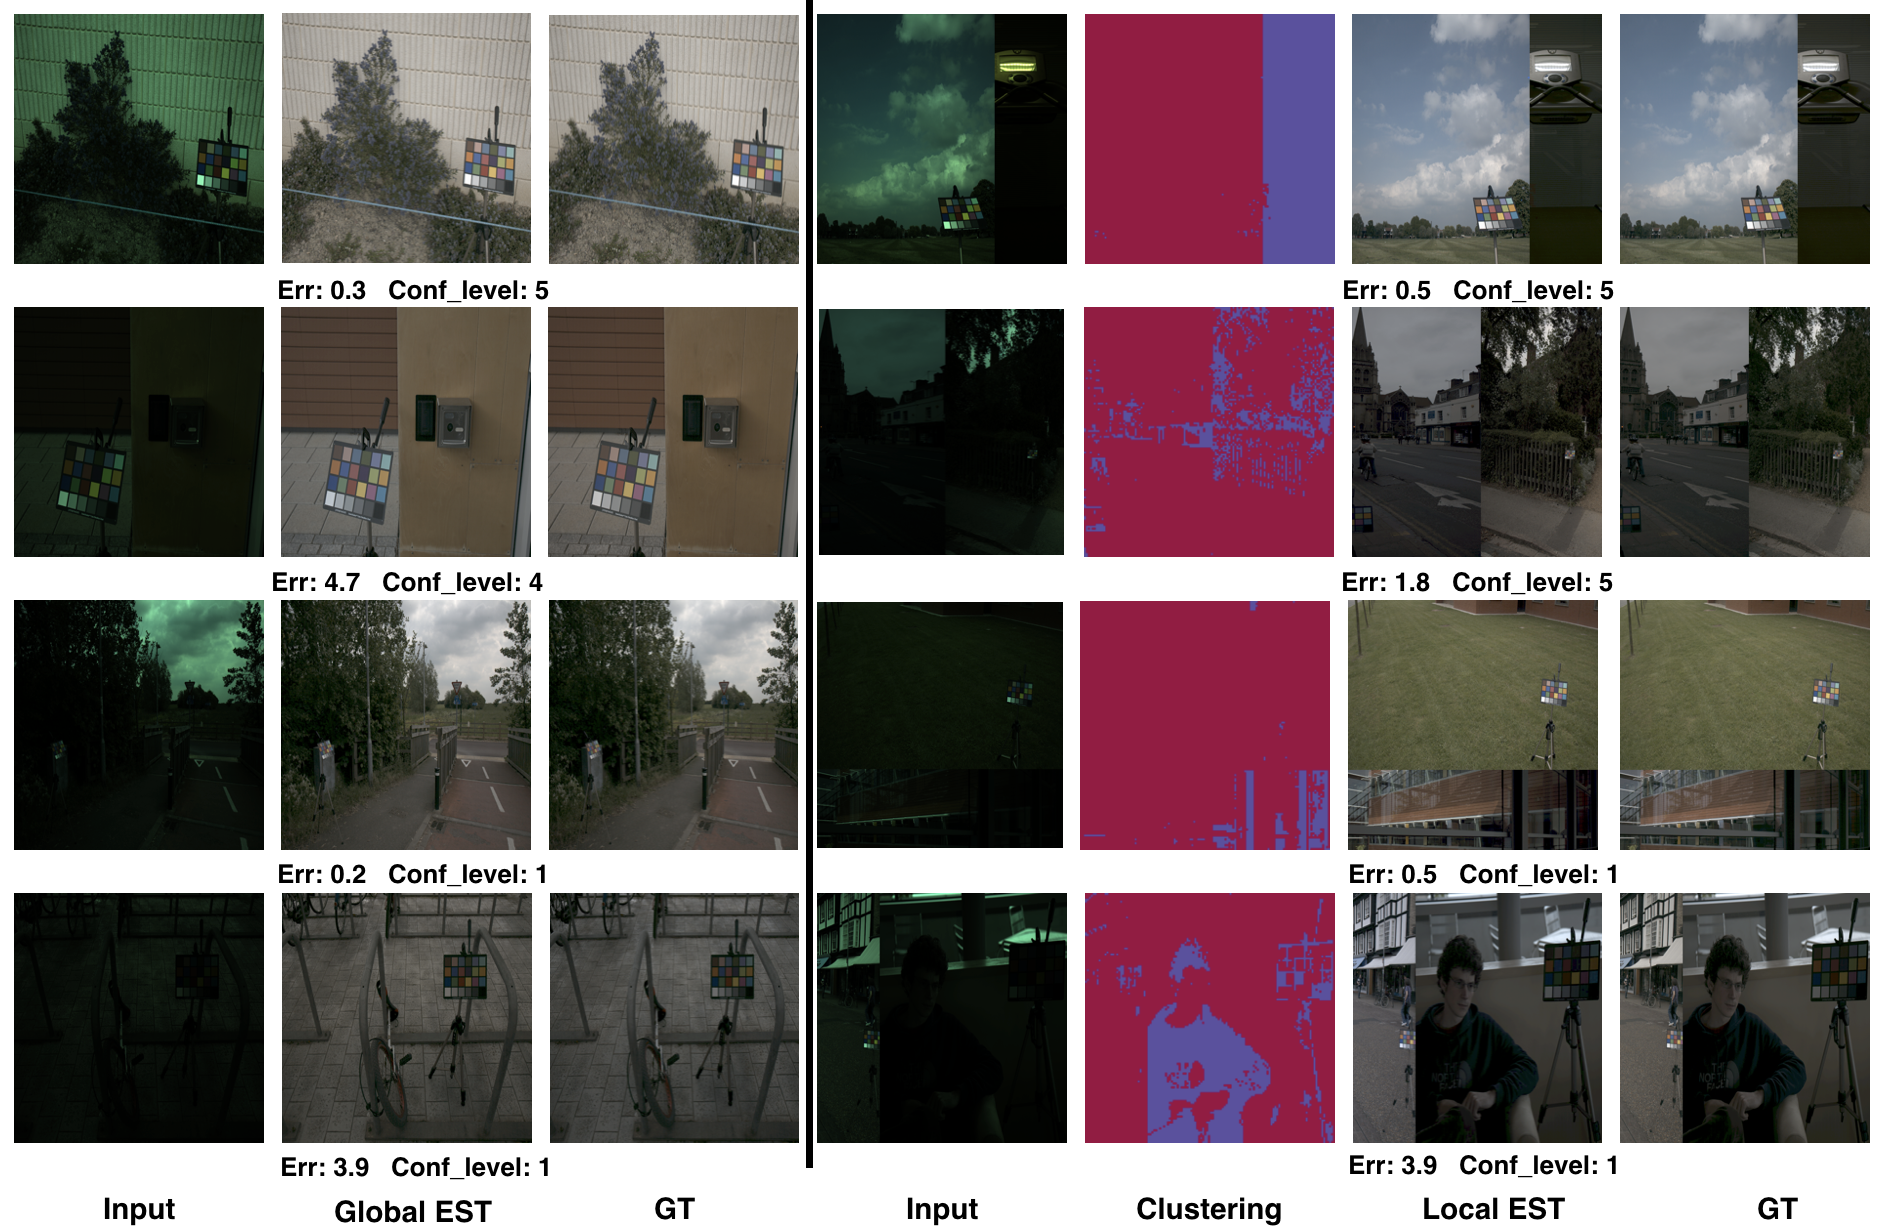
\includegraphics[width=1.0\textwidth]{../Images/all_0.png}
}
\subfigure {
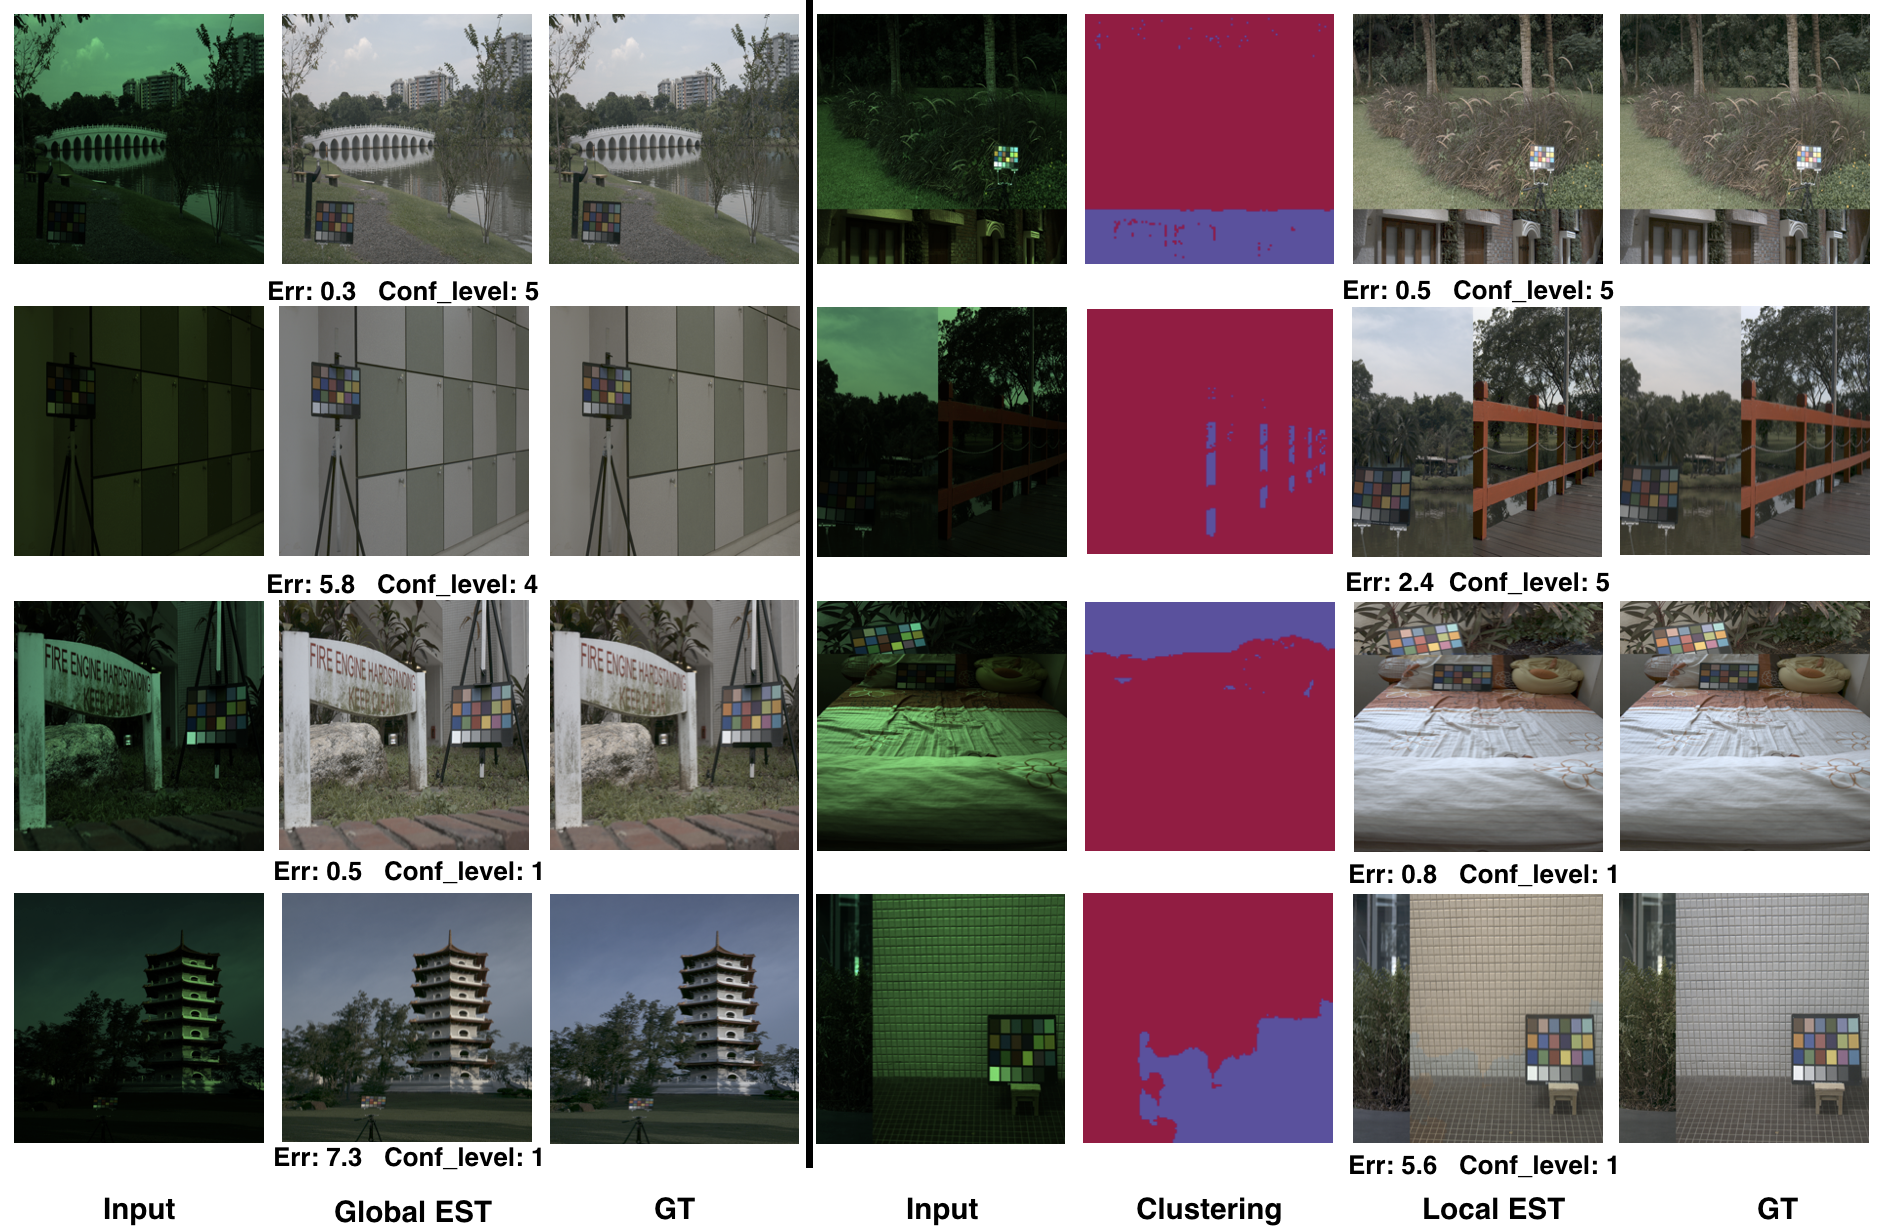
\includegraphics[width=1.0\textwidth]{../Images/all_1.png}
}
\end{center}
\caption{Examples of single (\textbf{left}) and multi-illuminant (\textbf{right}) White Balance (WB) results on Gehler and NUS-8 dataset.
        Single illuminant WB is based on global fitting.
        The top-down order is organized as high confidence, small error;
        high confidence, big error; low confidence, small error; low confidence big error.}
\label{fig:all_results_0}
\end{figure*}


\begin{figure*}
\begin{center}
% \fbox{\rule{0pt}{10in} \rule{.9\linewidth}{0pt}}
\subfigure {
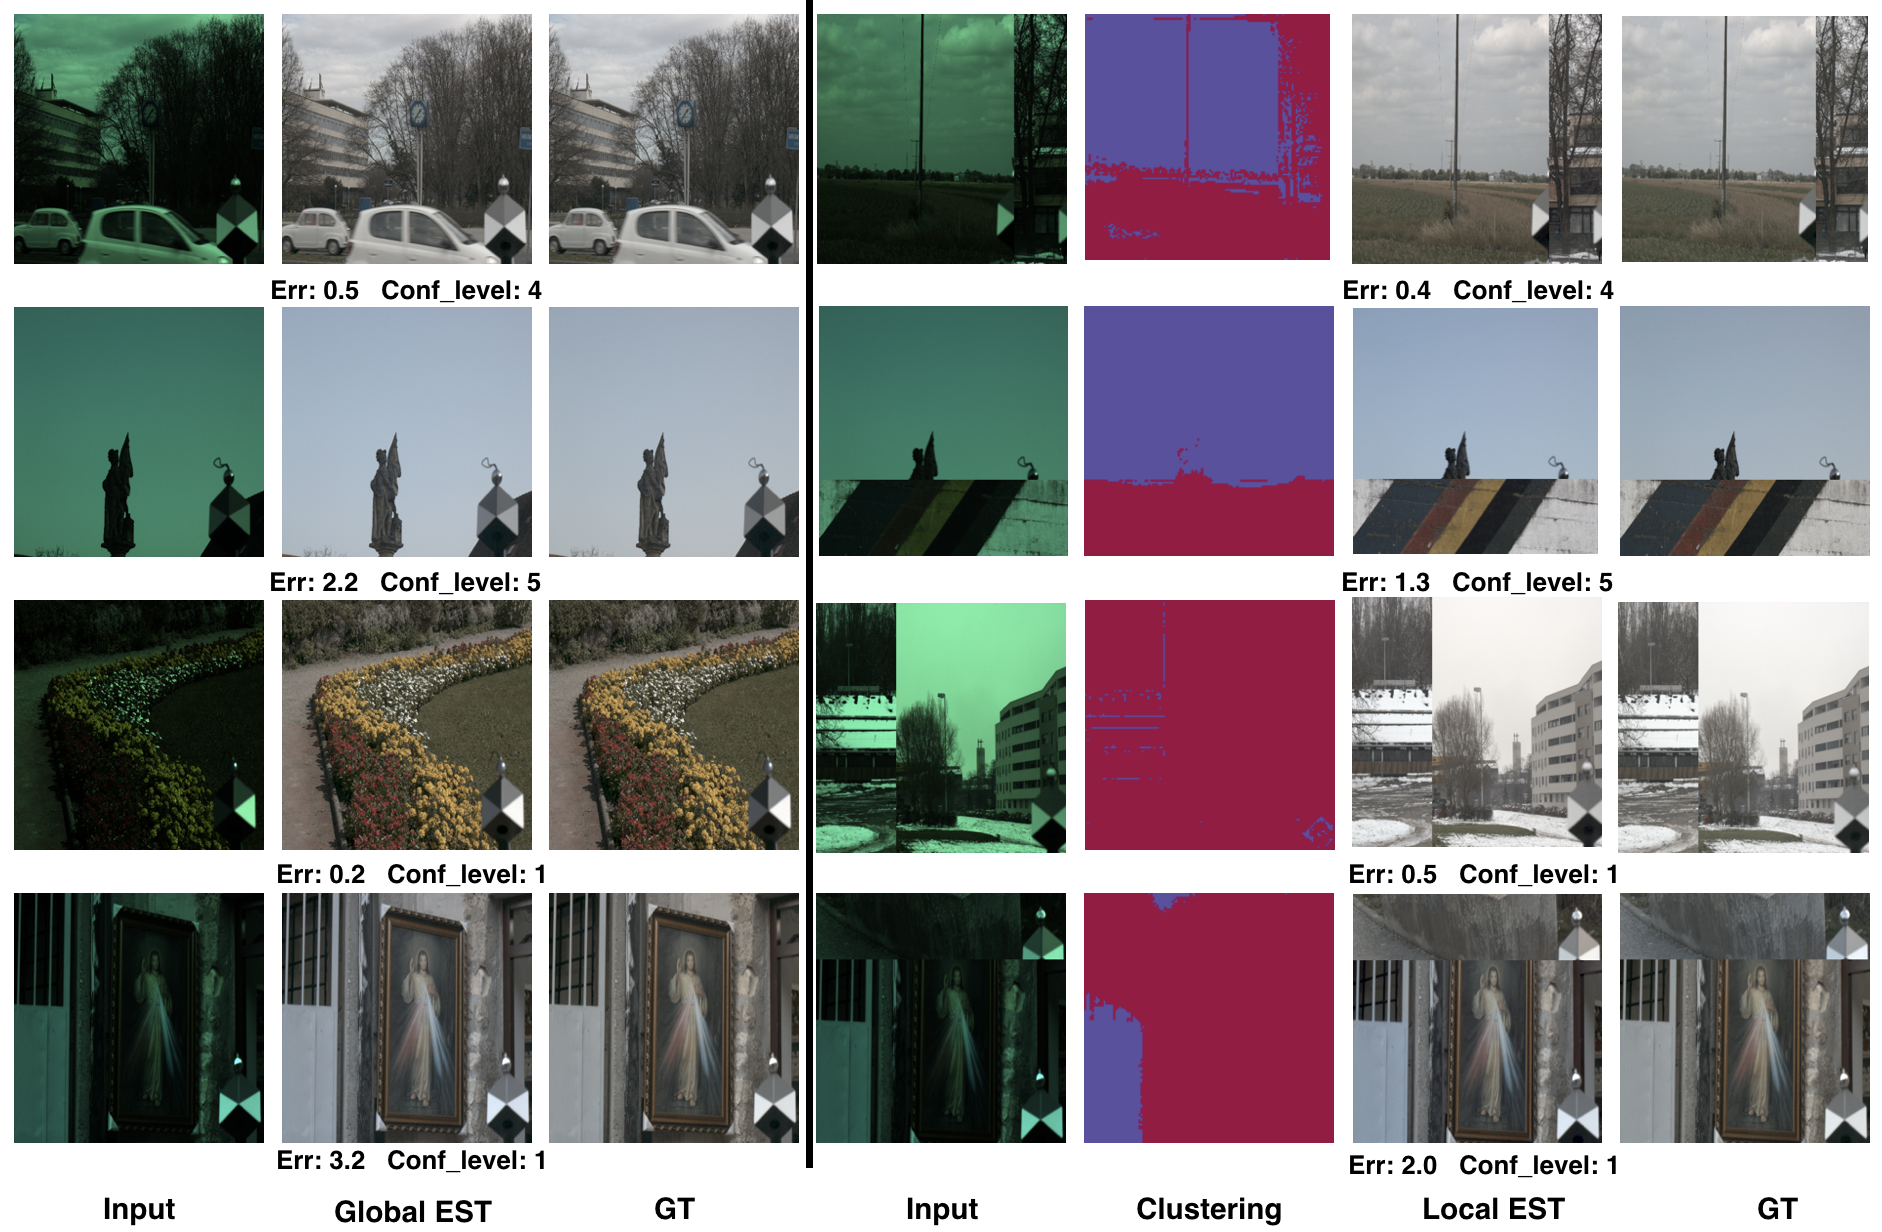
\includegraphics[width=1.0\textwidth]{../Images/all_2.png}
}
\subfigure {
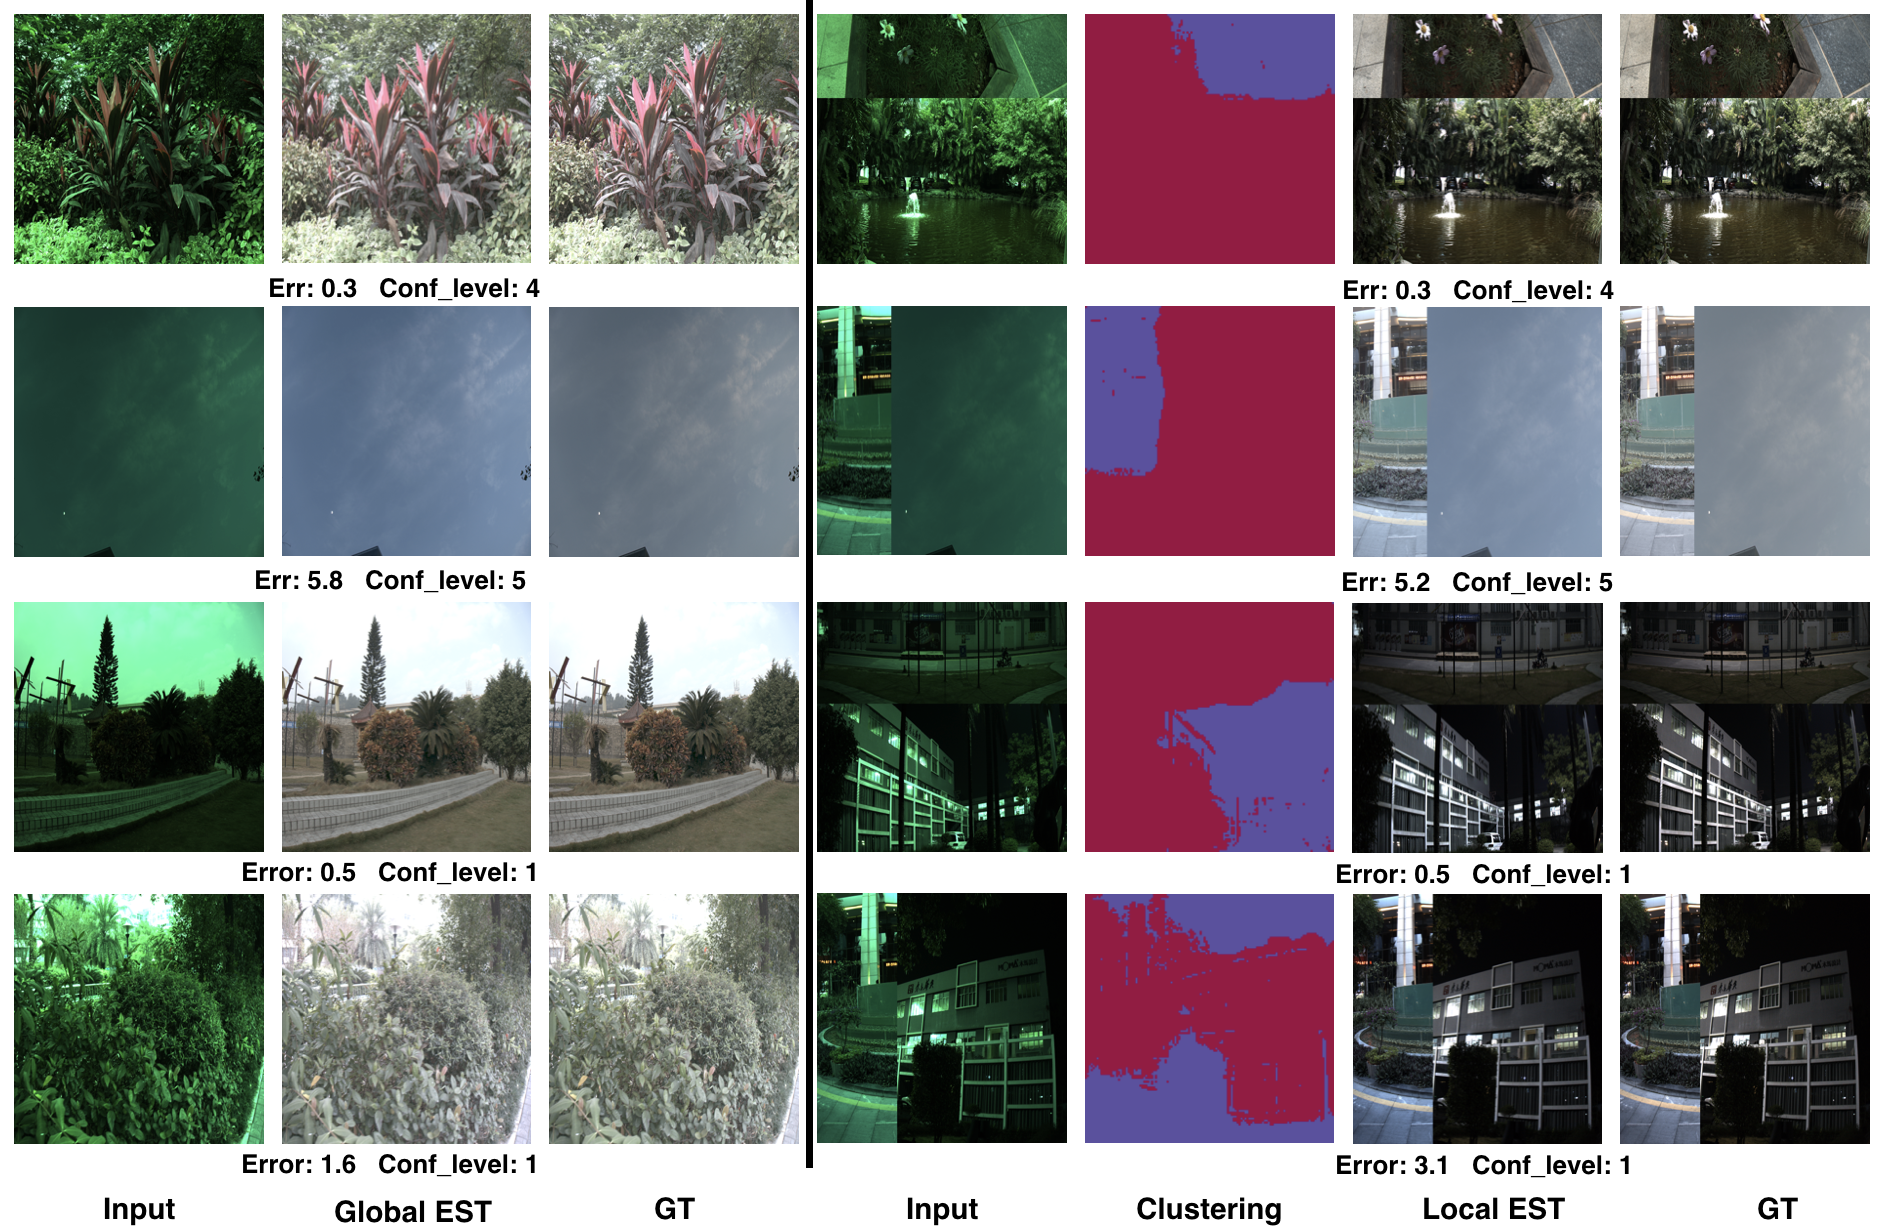
\includegraphics[width=1.0\textwidth]{../Images/all_3.png}
}
\end{center}
\caption{Examples of single (\textbf{left}) and multi-illuminant (\textbf{right}) WB results on Cube and MIO dataset,
        Single illuminant WB is based on global fitting.
        The top-down order is organized as high confidence, small error;
        high confidence, big error; low confidence, small error; low confidence big error.}
\label{fig:all_results_1}
\end{figure*}

% *********************

{\small
% \bibliographystyle{plain}
\bibliographystyle{ieee}
\bibliography{egbib}
}

\end{document}
